\documentclass{beamer}

\usepackage{ctex}
\usepackage{braket}
\usepackage{graphicx}
\graphicspath{{pics/}}
\usepackage{subfigure}  %插入子图用
\setbeamertemplate{caption}[numbered]  %让插入的图片自动编号(beamer默认不编号)
\usefonttheme{serif}   %在公式中使用使用标准的Latex字体(有衬线的字体),区分小的L和大写的I
%beamer中默认使用Sans Serif字体,即没有衬线的字体
\renewcommand{\thefootnote}{}    %取消脚注的编号,在后面花括号内添加其他符号也可改变脚注符号
\usepackage{caption}
\usepackage[english]{babel} % 将时间改成英
\usepackage{calligra}
\usepackage{xcolor}
\definecolor{custombg}{HTML}{DCE7E0}
\setbeamertemplate{navigation symbols}

% 修改beamer脚注的默认设置
\usepackage{etoolbox}  % 引入etoolbox以方便进行宏的修补
\makeatletter
\defbeamertemplate*{footnote}{nonumber}{
	\parindent 1em\noindent% 
	\raggedright
	\insertfootnotetext\par
}
\setbeamertemplate{footnote}[nonumber]  % 应用自定义的脚注模板
\makeatother

% 幻灯片字体和主题
\usepackage{times}
\usetheme{CambridgeUS}
\usecolortheme{spruce}

% 替换校徽
\pgfdeclareimage[height=0.6cm]{badge}{badge}
\logo{\pgfuseimage{badge}}

% 目录设置
\AtBeginSection[]{
	\begin{frame}
		\tableofcontents[currentsection]
	\end{frame}
}

% 首页信息
% \title[组会文献汇报]
\title[literature report]
{High-Resolution Image Synthesis with Latent Diffusion Models}

\author[Yingjian Zhu]
{\fontsize{8}{10}\selectfont
	San Zhang\inst{1,2}, Si Li\inst{2}, and Wu Wang\inst{3}
	\\[10pt]
	\href{mailto:zhangsan@ia.ac.cn}
	{Email: \textit{zhangsan@ia.ac.cn}}}

\institute[UCAS]
{\fontsize{6}{10}\selectfont
	\inst{1}School of Artificial Intelligence, University of Chinese Academy of Sciences\\
	\inst{2,3}Institute of Automation, Chinese Academy of Sciences}

% \date[\today]
\date[Nov 20, 2024]
{\fontsize{8}{10}
	\selectfont Nov 20, 2024}

% 正文
\begin{document}
	\logo{}
	\begin{frame}
		\titlepage
		\begin{center}
			\vspace{-15pt}
			
\includegraphics[width=0.3\linewidth]{Badge.pdf}
		\end{center}
	\end{frame}
	
	% 目录
	% \logo{\pgfuseimage{badge}}
	% \begin{frame}
	% 	\frametitle{Contents}
	% 	\tableofcontents
	% \end{frame}
	% \logo{}
	% 目录
    \logo{
\includegraphics[width=1.8cm,height=1.6cm]{figs/casia_logo.pic.jpg}}
	\begin{frame}
		\frametitle{Contents}
		\tableofcontents
	\end{frame}
	\logo{}
	
	
	
	
	
	% Section 1
	\section[Introduction]{Introduction}
	\begin{frame}
		\frametitle{The Development of AI-Generated Content (AIGC)}
		\begin{figure}[t]
			\centering
			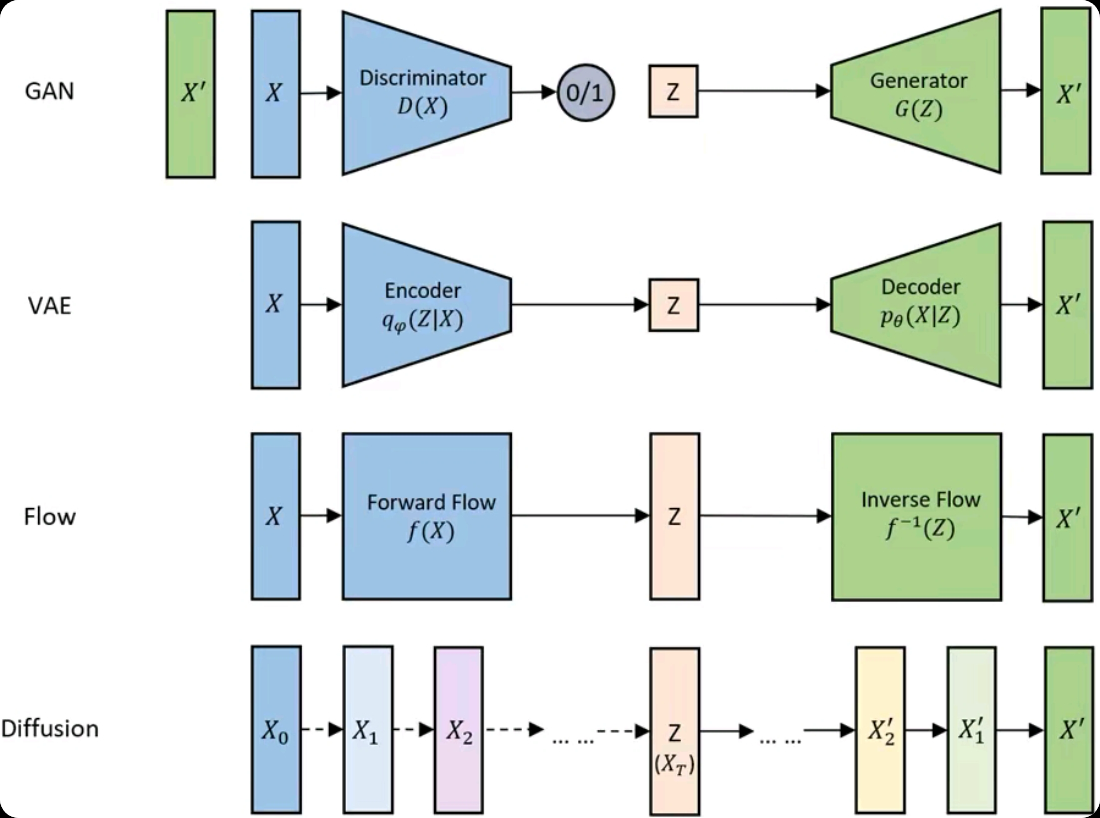
\includegraphics[width=3in]{figs/fig1.png}
			\vspace{0mm}
			\captionsetup{font=scriptsize}
			\caption{The development of AIGC and mobile edge computing network [1].}
			\vspace{0mm}
		\end{figure}
		\footnotetext{\noindent \tiny [1] M. Xu, \emph{et al.}, ``Unleashing the power of edge-cloud generative AI in mobile networks: A survey of AIGC services,'' \emph{IEEE Commun. Surv. Tutor.}, Early Access, 2024.}
	\end{frame}


	\begin{frame}
		\frametitle{Diffusion Model}
		\begin{figure}[t]
			\centering
			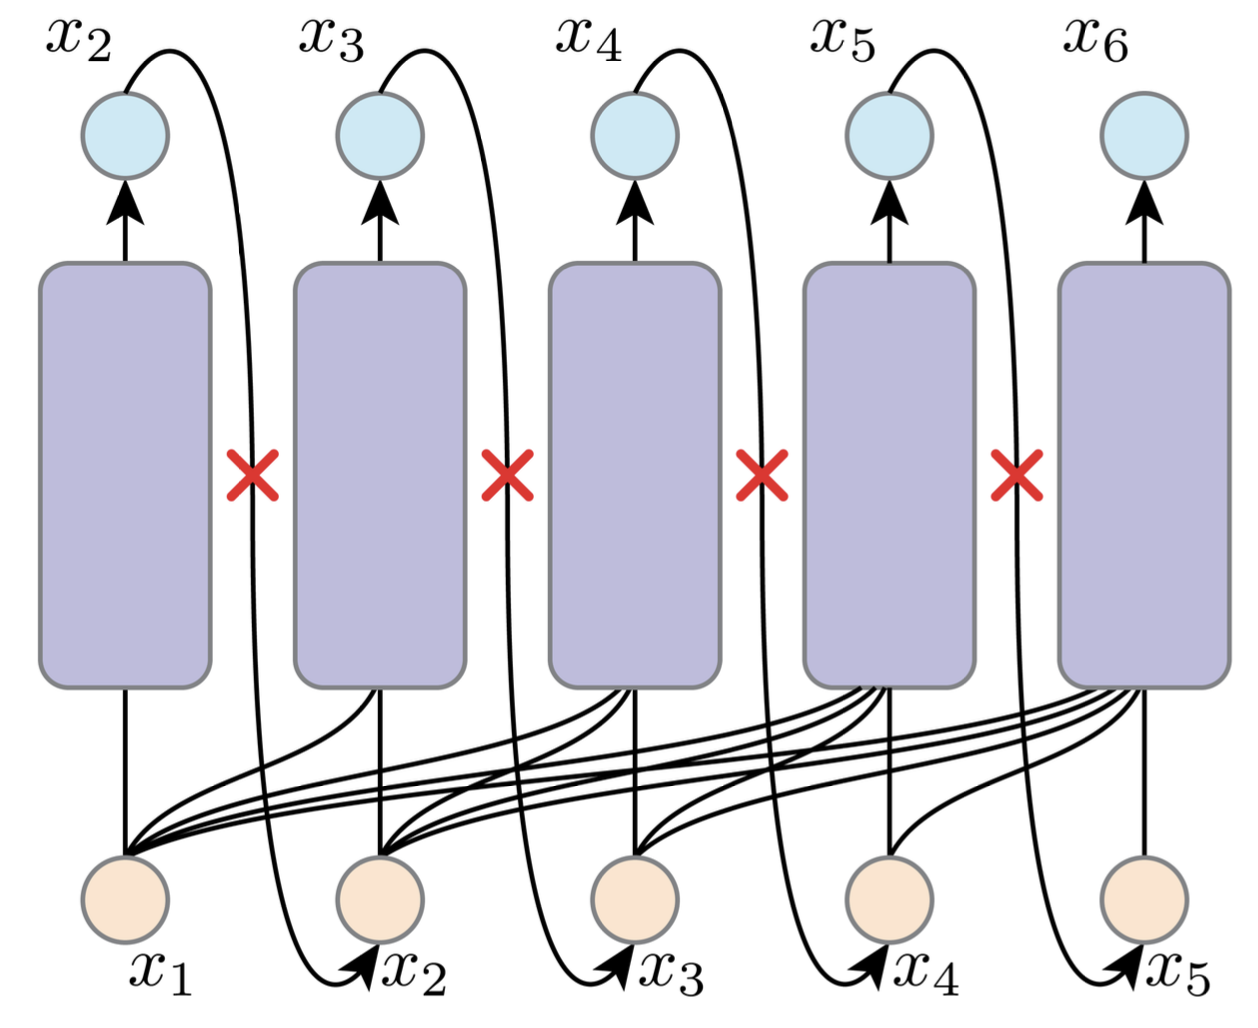
\includegraphics[width=2in]{figs/fig2.png}
			\vspace{0mm}
			\captionsetup{font=scriptsize}
			\caption{An illustration of diffusion model [2].}
			\vspace{-2mm}
		\end{figure}
		\begin{itemize}
			\item With Gaussian noise as input
			\item The quality of generated images gets progressively better.
		\end{itemize}
		\footnote{\noindent \tiny{[2] H. Du, \emph{et al.}, ``Enhancing deep reinforcement learning: A tutorial on generative diffusion models in network optimization," \emph{arXiv preprint arXiv:2308.05384}, 2023.}}
	\end{frame}
	
	
	\begin{frame}
	\frametitle{AIGC in Mobile Edge Computing (MEC)}
		\begin{figure}[t]
			\centering
			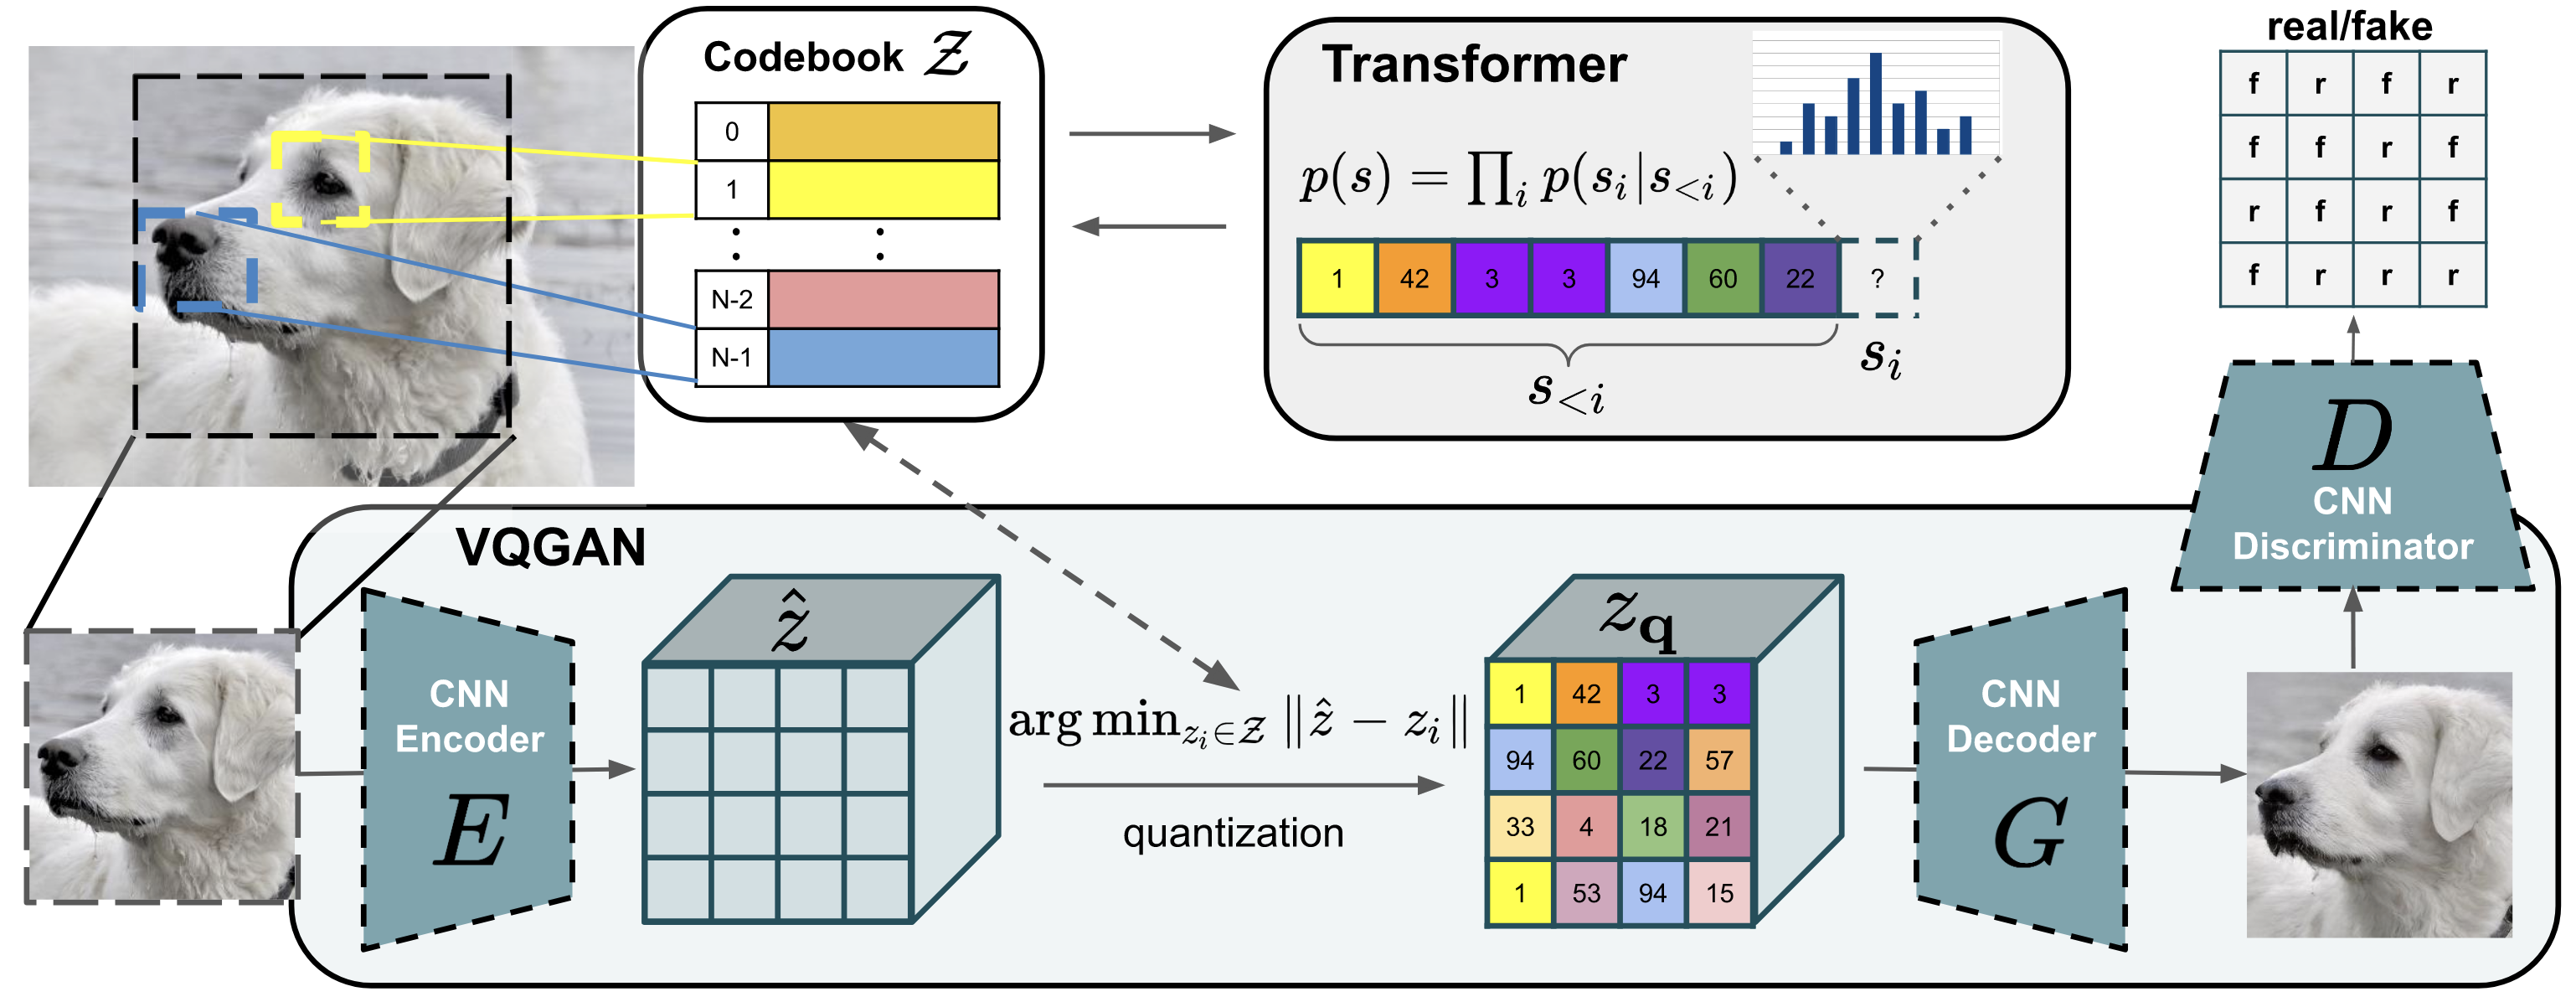
\includegraphics[width=3.6in]{figs/fig3.png}
			\vspace{0mm}
			\captionsetup{font=scriptsize}
			\caption{An overview of a mobile AIGC network [1].}
			\vspace{0mm}
		\end{figure}
		\begin{itemize}
			\vspace{-3mm}
			\item AIGC models can be deployed at edge servers.
		\end{itemize}
		\footnotetext{\noindent \tiny [1] M. Xu, \emph{et al.}, ``Unleashing the power of edge-cloud generative AI in mobile networks: A survey of AIGC services,'' \emph{IEEE Commun. Surv. Tutor.}, Early Access, 2024.}
	\end{frame}

	
	
	
	
	% Section 2
	\section[System Model]{System Model}
	\subsection{Network Model}
	\begin{frame}
		\frametitle{MEC Network}
	\end{frame}
	
	
	\subsection{Task Processing Model}
	\begin{frame}
		\frametitle{Local Processing Model}
	\end{frame}
	
	
	\begin{frame}
		\frametitle{Home BS Processing Model}
	\end{frame}
	
	
	\begin{frame}
		\frametitle{Neighbor BS Processing Model}
	\end{frame}
	
	
	
	
	
	% Section 3
	\section[Problem Formulation]{Problem Formulation}
	\begin{frame}
		\frametitle{Weighted Cost}
	\end{frame}


	\begin{frame}
		\frametitle{Offloading Problem}
	\end{frame}





	% Section 4
	\section[Algorithm Design]{Algorithm Design}
	\begin{frame}
		\frametitle{Deep Reinforcement Learning based OSI Algorithm}
		\begin{itemize}
			\item State:
			$$
			\bold{s}_n^{(l)} = \left( B_n^{(l)}, q_n^{(l)}, f_n^{\text{U},(l)}, \bold{g}^{\text{B},(l)}, \bold{h}_n^{(l)} \right)
			$$
			\item Action:
			$$
			\bold{a}_n^{(l)} = \left( x_n^{(l)}, \bold{y}_{n}^{(l)}, c_n^{(l)} \right)
			$$
			\item Reward:
			$$
			r_n^{(l)} = -\sum_{n \in \mathcal{N}} \left( \omega_1 T_n^{(l)} + \omega_2 E_n^{(l)} + \omega_3 \epsilon_n^{(l)} \right)-r_n^{\text{P},(l)}
			$$
		\end{itemize}
	\end{frame}





	% Section 5
	\section[Simulation Results]{Simulation Results}
	\begin{frame}
	\end{frame}





	% Section 6
	\section[Conclusion]{Conclusion}
	\begin{frame}
		\begin{itemize}
			\item Conclusion 1.
			\item Conclusion 2.
			\item Conclusion 3.
			\item Conclusion 4.
		\end{itemize}
	\end{frame}


	\section{}
	\logo{\pgfuseimage{badge}}
	\begin{frame}{Acknowledgements}
		\begin{center}
			\begin{minipage}{1\textwidth}
				\setbeamercolor{mybox}{fg=black, bg=custombg}
				\begin{beamercolorbox}[wd=0.6\textwidth, rounded=true, shadow=true]{mybox}
					\LARGE \centering Thanks for your listening!
				\end{beamercolorbox}
			\end{minipage}
			\\[20pt]
			Please feel free to contact us:
			\\[10pt]
			\textit{zhangsan@ia.ac.cn}
		\end{center}
	\end{frame}

\end{document}